\documentclass[conference]{IEEEtran}

\usepackage{cite}
\usepackage{amsmath,amssymb,amsfonts}
\usepackage{algorithmic}
\usepackage{graphicx}
\usepackage{textcomp}
\usepackage{xcolor}

\usepackage{url}    % Per creare url


\begin{document}

\title{HVAC Waste Detection - Project Report}

\author{\IEEEauthorblockN{Daniele Polidori}
\IEEEauthorblockA{\textit{Course of Internet of things}\\
\textit{University of Bologna}\\
Academic year 2023-24\\
daniele.polidori2@studio.unibo.it}}

\maketitle


\section{Introduction}
I implemented an IoT system that monitors the temperature of an house, to prevent useless HVAC consumption, detecting it by rapid temperature changes\footnote{\url{https://github.com/danielepolidori/HVAC_Waste_Detection}}. Reducing energy usage has good environmental reasons and also saves money on the bills.\\
In this report, I show the components and the structure of the system I've realized. Then I show the experimental setup and the consequent results I've obtained; at the end, I present some thoughts on them.


\section{Project’s Architecture}
The system is composed by an ESP-WROOM-32 board linked to two DHT22 sensors (one positioned indoor, near air exits, and one outdoor) and to a LED, as in Fig.~\ref{fig_esp}.\\
The board periodically collects indoor and outdoor temperature values. They are constantly analysed: if the indoor temperature values rapidly change (approaching the outdoor values) the LED is temporarily turned on, thus showing an alarm signal to the user. In this way, if the temperature change is caused by, e.g., an open window, it can be saved unnecessary HVAC waste. At the beginning, based on all past temperature data, the system predicts some future temperature values.\\
The collected temperature data are continuously sent to a gateway, that stores them, together with the alarm triggers and the forecasted temperature values, on a local time-series database. All data are interactively visualized by a local web application, that shows them by means of charts, as in Fig.~\ref{fig_grafana}.

\begin{figure}[htbp]
    \centerline{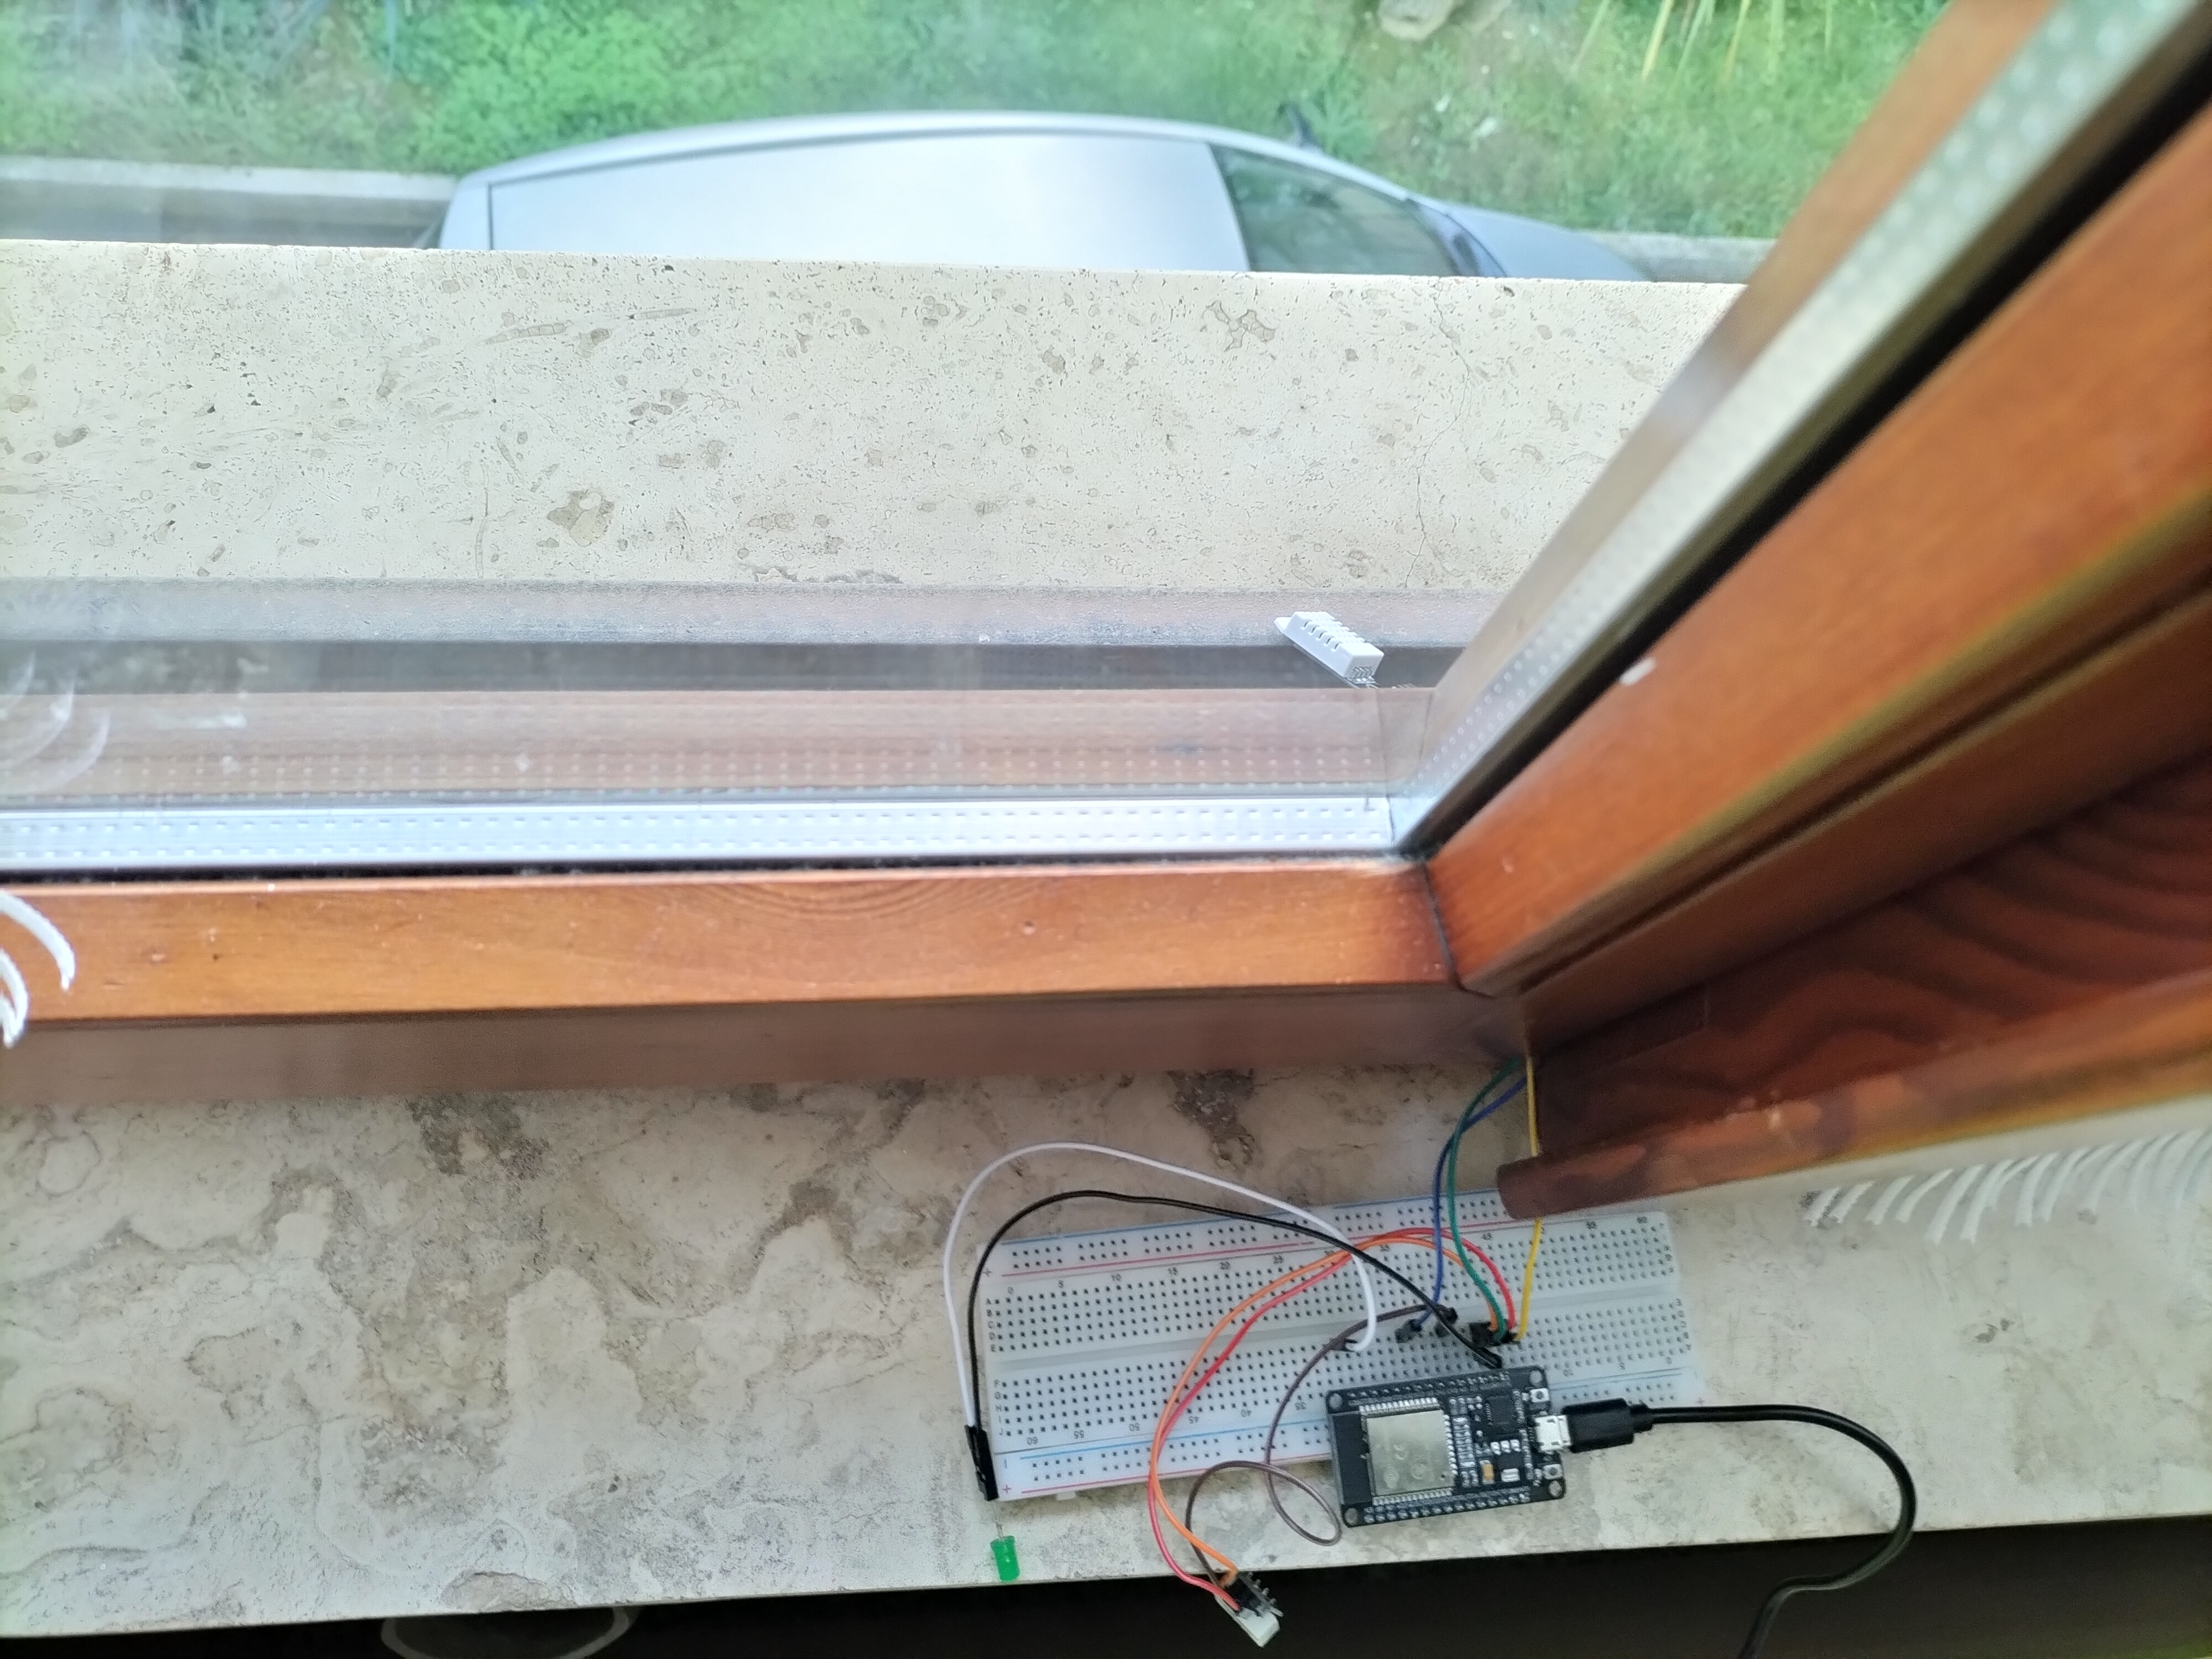
\includegraphics[scale=0.06]{figures/figure_esp.jpg}}
    \caption{ESP32 board linked to two DHT22 sensors and to a LED.}
    \label{fig_esp}
\end{figure}

\begin{figure}[htbp]
    \centerline{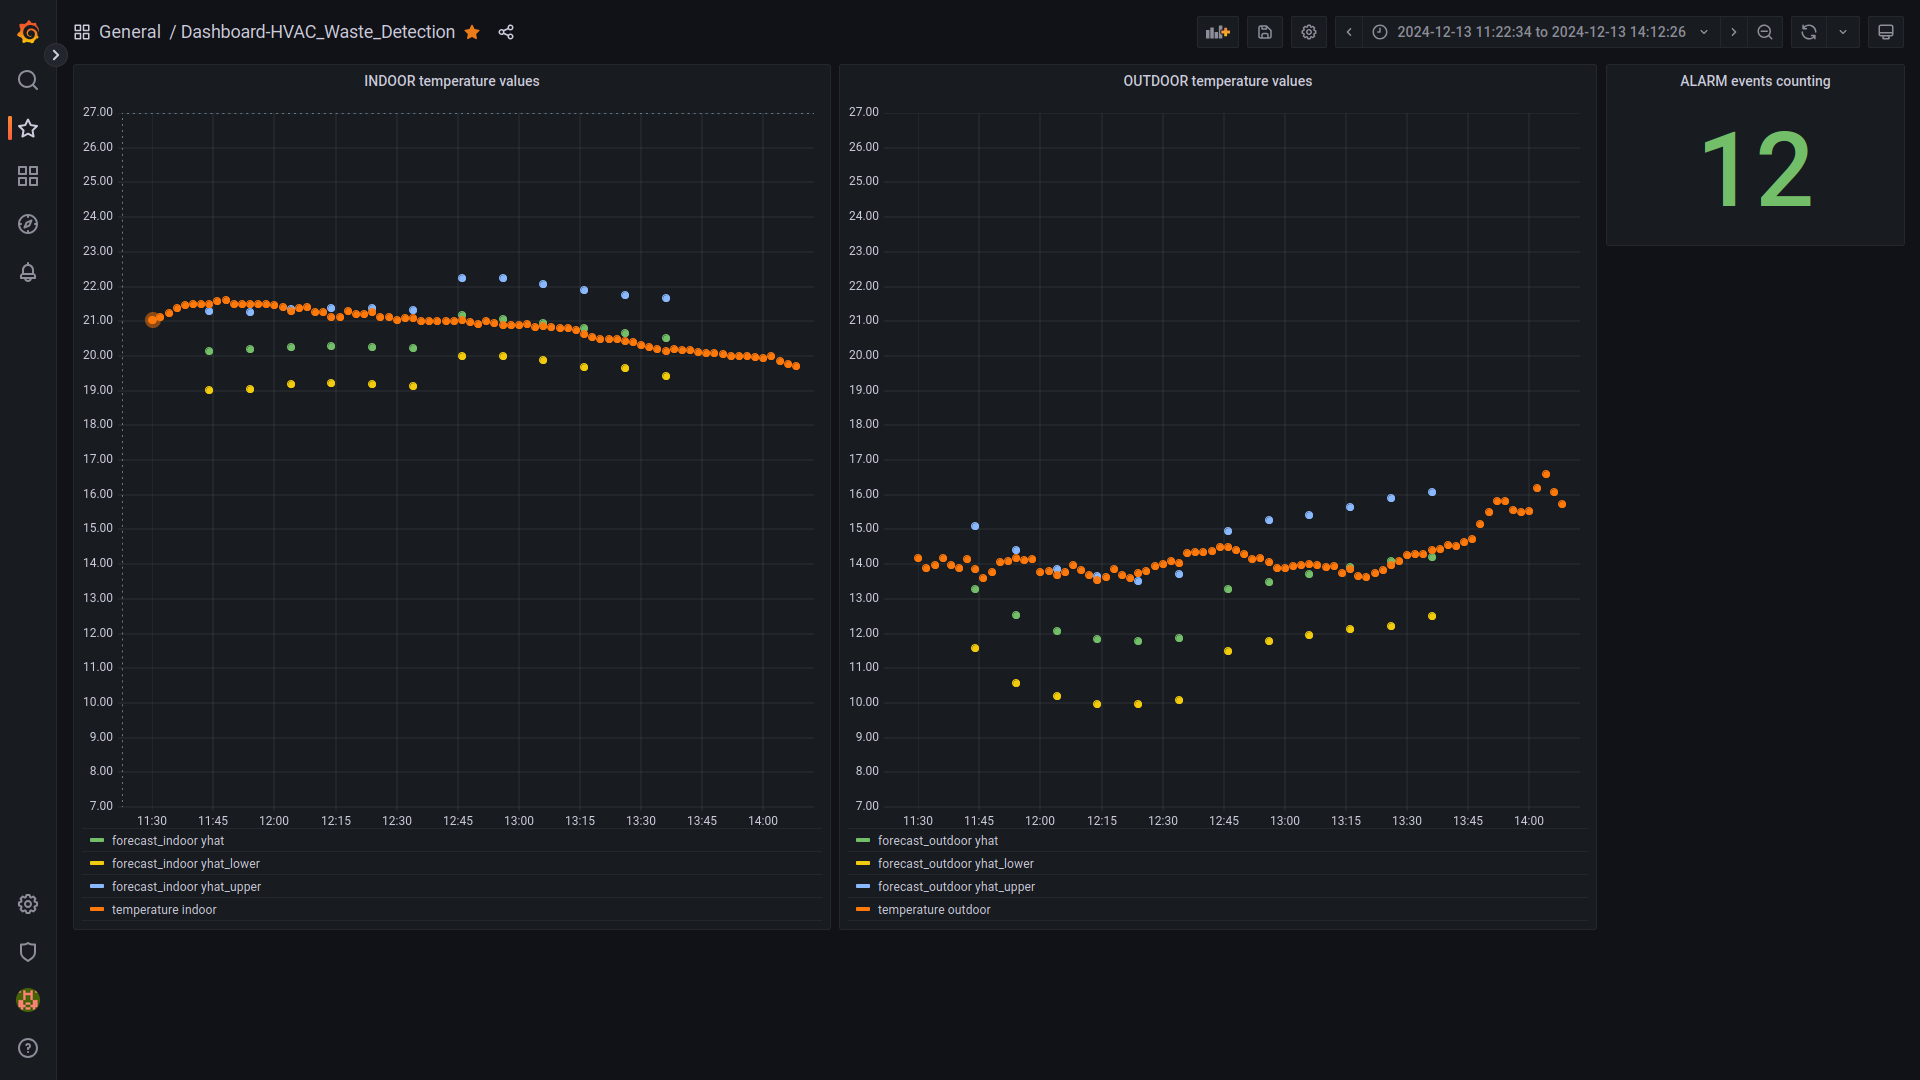
\includegraphics[scale=0.125]{figures/figure_grafana.png}}
    \caption{Dashboard on Grafana, showing the collected data.}
    \label{fig_grafana}
\end{figure}


\section{Project’s Implementation}

\subsection{Data acquisition}
I made the \texttt{data\_acquisition.ino} file to program the ESP32 board. I use the \texttt{Thing.CoAP} library to make the board act as a CoAP server and the \texttt{PubSubClient} library to make it act as a MQTT subscriber.\\
Through the CoAP protocol, the ESP32 is able to send the latest collected indoor and outdoor temperature value, when asked.\\
Through the MQTT protocol, the board can receive some commands: to start or stop the sensors reading (at the beginning they are off), to change the interval between consecutive sensors readings --- in both cases, it can be considered just one of the two sensors --- and to turn on or off the LED. My laptop acts as a MQTT broker, through Mosquitto.

\subsection{Data proxy}
I made the \texttt{data\_proxy.py} file to create a Python application. I use the \texttt{paho-mqtt} library to make the script act as a MQTT publisher, the \texttt{aiocoap} library to make it act as a CoAP client and the \texttt{influxdb-client} library to store data.\\
Initially, through the MQTT protocol, the application gives commands, to the ESP32, to start the sensors reading and to set their sampling rate.\\
Periodically, through the CoAP protocol, the script requests, to the board, the latest collected indoor and outdoor temperature value. It continuously stores these values on a local InfluxDB instance.\\
The network latency, between the temperature value request (from the application to the ESP32) and its reception, is continuously monitored; after a while from the beginning, the script evaluates the mean latency of this process.

\subsection{Data analytics}
I made the \texttt{data\_analytics.py} file to create another Python application. I use the \texttt{influxdb-client} library to get and store data on the database, the \texttt{prophet} library to forecast future temperature values and the \texttt{paho-mqtt} library to make it act as a MQTT publisher.\\
At the beginning, the script gets all past temperature values from the database to make a prediction of some indoor and outdoor future values. As the forecasted temperature times are reached, the application stores the predicted values on the database.\\
Ciclically, the application retrieves some of the latest temperature values from the database and analyses them to check a possible HVAC waste. The alarm goes off if the variance of the latest indoor temperature values is above a certain threshold \eqref{eq_varianza} (i.e. if the indoor temperature is changing rapidly) and if the mean of them is between the farthest of the latest indoor temperature values and the farthest of the latest outdoor ones \eqref{eq_media} (i.e. if the indoor temperature is approaching the outdoor one). Mathematically speaking:
\begin{equation}
var(i_1, i_2, \dots, i_n) > threshold \label{eq_varianza}
\end{equation}
\begin{equation}
min(i_n, o_n) < mean(i_1, i_2, \dots, i_n) < max(i_n, o_n) \label{eq_media}
\end{equation}
where $i$ is the indoor temperature, $o$ is the outdoor temperature and $t_1, t_2, \dots, t_n$ are the $n$ latest temperature values retreived: $t_1$ is the newest and $t_n$ is the farthest. When the alarm goes off, the script stores the alarm event on the database and, through the MQTT protocol, gives the command, to the ESP32, to turn on the LED; when the risk has passed, the script gives the command to turn it off.\\
The collected temperature values, together with the forecasted ones, and the counting of the alarm events are always shown on a local Grafana instance, by means of a dashboard, as in Fig.~\ref{fig_grafana}.


\section{Results}

\subsection{Setup}
To evaluate the performance of the system, I've experimented the following setup.\\
The data proxy application sets the indoor sensor to collect data every 3 seconds and the outdoor one every 20 seconds; it asks for the latest indoor and outdoor temperature value every 5 seconds. The mean network latency is evaluated after 1 hour from the beginning.\\
The data analytics script, initially, retrieves all past temperature data from the database, unevenly collected during the past month, for the forecasting, aggregating them every 20 seconds by the mean function: in this way, it gets more than 6500 indoor temperature values and as many outdoor. The application makes a prediction about the temperature of the next hour: it forecasts an indoor and an outdoor value every 10 minutes, for 6 times. Furthermore, every 30 seconds, the script retrieves the temperature values of the latest 2 minutes, without aggregating them, for the alarm check: the threshold, seen in \eqref{eq_varianza}, is $0.03$.

\subsection{Evaluation}
I started the data proxy application at 11:30 on December 13th and the data analytics script at 12:36. The forecasted temperature values, compared with the observed ones, are shown in Tab.~\ref{tab_forecast_indoor} (the indoor ones), in Tab.~\ref{tab_forecast_outdoor} (the outdoor ones) and in Fig.~\ref{fig_grafana}. It's considered, as observed temperature, the mean value  of the temperatures collected during the minute before and after the forecasted temperature time. The mean network latency of the data acquisition process was $150$ milliseconds, with values ranging from $5$ to $421$.\\
The results are pretty good: the forecasted values differ from the observed ones by a maximum of $0.39$ °C for the indoor temperature and of $1.23$ °C for the outdoor one; in any case they are always within the forecasted range. The system is a little more reliable in forecasting the indoor temperature. It can be due to the higher sampling rate of the indoor sensor: this choice arises from the fact that it's useful in order to rapidly detect an eventual HVAC waste, while it's unnecessary outdoor.\\
The experiment has limitations: there wasn't many past temperature values available and they were collected unevenly. Furthermore, the ESP32 was positioned in a naive way (Fig.~\ref{fig_esp}): it should be arranged in such a way as to avoid direct sunlight.

\begin{table}[htbp]
    \caption{Indoor Temperature Forecast Evaluation}
    \begin{center}
        \begin{tabular}{|r|c|c|c|c|}
            \hline
            \textbf{Current} & \textbf{Observed}$^{\mathrm{a}}$ & \multicolumn{3}{|c|}{\textbf{Forecasted Temperature (°C)}} \\
            \cline{3-5}
            \textbf{Time} & \textbf{Temperature (°C)} & \textbf{\textit{yhat}} & \textbf{\textit{yhat lower}} & \textbf{\textit{yhat upper}} \\
            \hline
            12:46 & $21.04$ & \textbf{21.17} & $19.99$ & $22.25$ \\
            \hline
            12:56 & $20.88$ & \textbf{21.07} & $19.98$ & $22.24$ \\
            \hline
            13:06 & $20.85$ & \textbf{20.95} & $19.88$ & $22.06$ \\
            \hline
            13:16 & $20.63$ & \textbf{20.81} & $19.69$ & $21.90$ \\
            \hline
            13:26 & $20.42$ & \textbf{20.66} & $19.66$ & $21.77$ \\
            \hline
            13:36 & $20.13$ & \textbf{20.52} & $19.43$ & $21.67$ \\
            \hline
            \multicolumn{4}{l}{$^{\mathrm{a}}$Mean temperature value (of the 2 minutes around).}
        \end{tabular}
        \label{tab_forecast_indoor}
    \end{center}
\end{table}

\begin{table}[htbp]
    \caption{Outdoor Temperature Forecast Evaluation}
    \begin{center}
        \begin{tabular}{|r|c|c|c|c|}
            \hline
            \textbf{Current} & \textbf{Observed}$^{\mathrm{a}}$ & \multicolumn{3}{|c|}{\textbf{Forecasted Temperature (°C)}} \\
            \cline{3-5}
            \textbf{Time} & \textbf{Temperature (°C)} & \textbf{\textit{yhat}} & \textbf{\textit{yhat lower}} & \textbf{\textit{yhat upper}} \\
            \hline
            12:46 & $14.50$ & $13.27$ & $11.49$ & \textbf{14.97} \\
            \hline
            12:56 & $14.07$ & \textbf{13.49} & $11.78$ & $15.26$ \\
            \hline
            13:06 & $14.01$ & \textbf{13.71} & $11.95$ & $15.42$ \\
            \hline
            13:16 & $13.86$ & \textbf{13.92} & $12.13$ & $15.65$ \\
            \hline
            13:26 & $13.98$ & \textbf{14.09} & $12.21$ & $15.91$ \\
            \hline
            13:36 & $14.40$ & \textbf{14.21} & $12.49$ & $16.09$ \\
            \hline
            \multicolumn{4}{l}{$^{\mathrm{a}}$Mean temperature value (of the 2 minutes around).}
        \end{tabular}
        \label{tab_forecast_outdoor}
    \end{center}
\end{table}


\end{document}
